\chapter{Combinatorial Analysis}

\section{Why combinatorial analysis?}

A communication system consist of \(n\) seemingly identical antennas that are lined up in a linear ordered array. The resulting system will then be able to receive all incoming signals and will be called functional as long as no two consecutive antennas are defective. If \(m\) of the \(n\) antennas are defective, how many different states of the system are possible?

If \(n =4\) and \(m=2\) there are \(6\) states possible : 

\[ 
\begin{matrix}
    0 & 1 & 1 & 0 \\
    1 & 0 & 1 & 0 \\
    1 & 0 & 0 & 1 \\
    0 & 1 & 0 & 1 \\
    0 & 0 & 1 & 1 \\
    1 & 1 & 0 & 0 \\
\end{matrix}
\]

In \(6\) of these \(3\) of them are functional. 

\begin{definition}
    The mathematical theory of counting is known as \textbf{combinatorial analysis}  
\end{definition}

\section{The basic principle of counting}

\begin{definitionbox}[title=The Basic Principle of Counting]
    Suppose that two experiments are to be performed. The first experiment has \(m\) possible outcomes and for each of these outcomes the second experiment has \(n\) possible outcomes. Then the two experiments together have \(m \times n\) possible outcomes.
\end{definitionbox}
\begin{examplebox}[title=Example: Coin and Die]
    A coin is tossed and a die is rolled. How many possible outcomes are there?
    
    \textbf{Solution:} The coin has \(2\) possible outcomes and the die has \(6\) possible outcomes. Therefore the two experiments together have \(2 \times 6 = 12\) possible outcomes.
\end{examplebox}


\begin{definitionbox}[title=The Generalized Basic Principle of Counting]
    If \(r\) experiments are to be performed are to be such that the first one may result in any of \(n_1\) possible outcomes, and for each of these \(n_{1}\) possible outcomes there are \(n_2\) possible outcomes for the second experiment, and so on up to the \(r\)-th experiment which may result in any of \(n_r\) possible outcomes, then the \(r\) experiments together have \(n_1 \times n_2 \times \ldots \times n_r\) possible outcomes.
\end{definitionbox}


\begin{figure}[H]
    \centering
    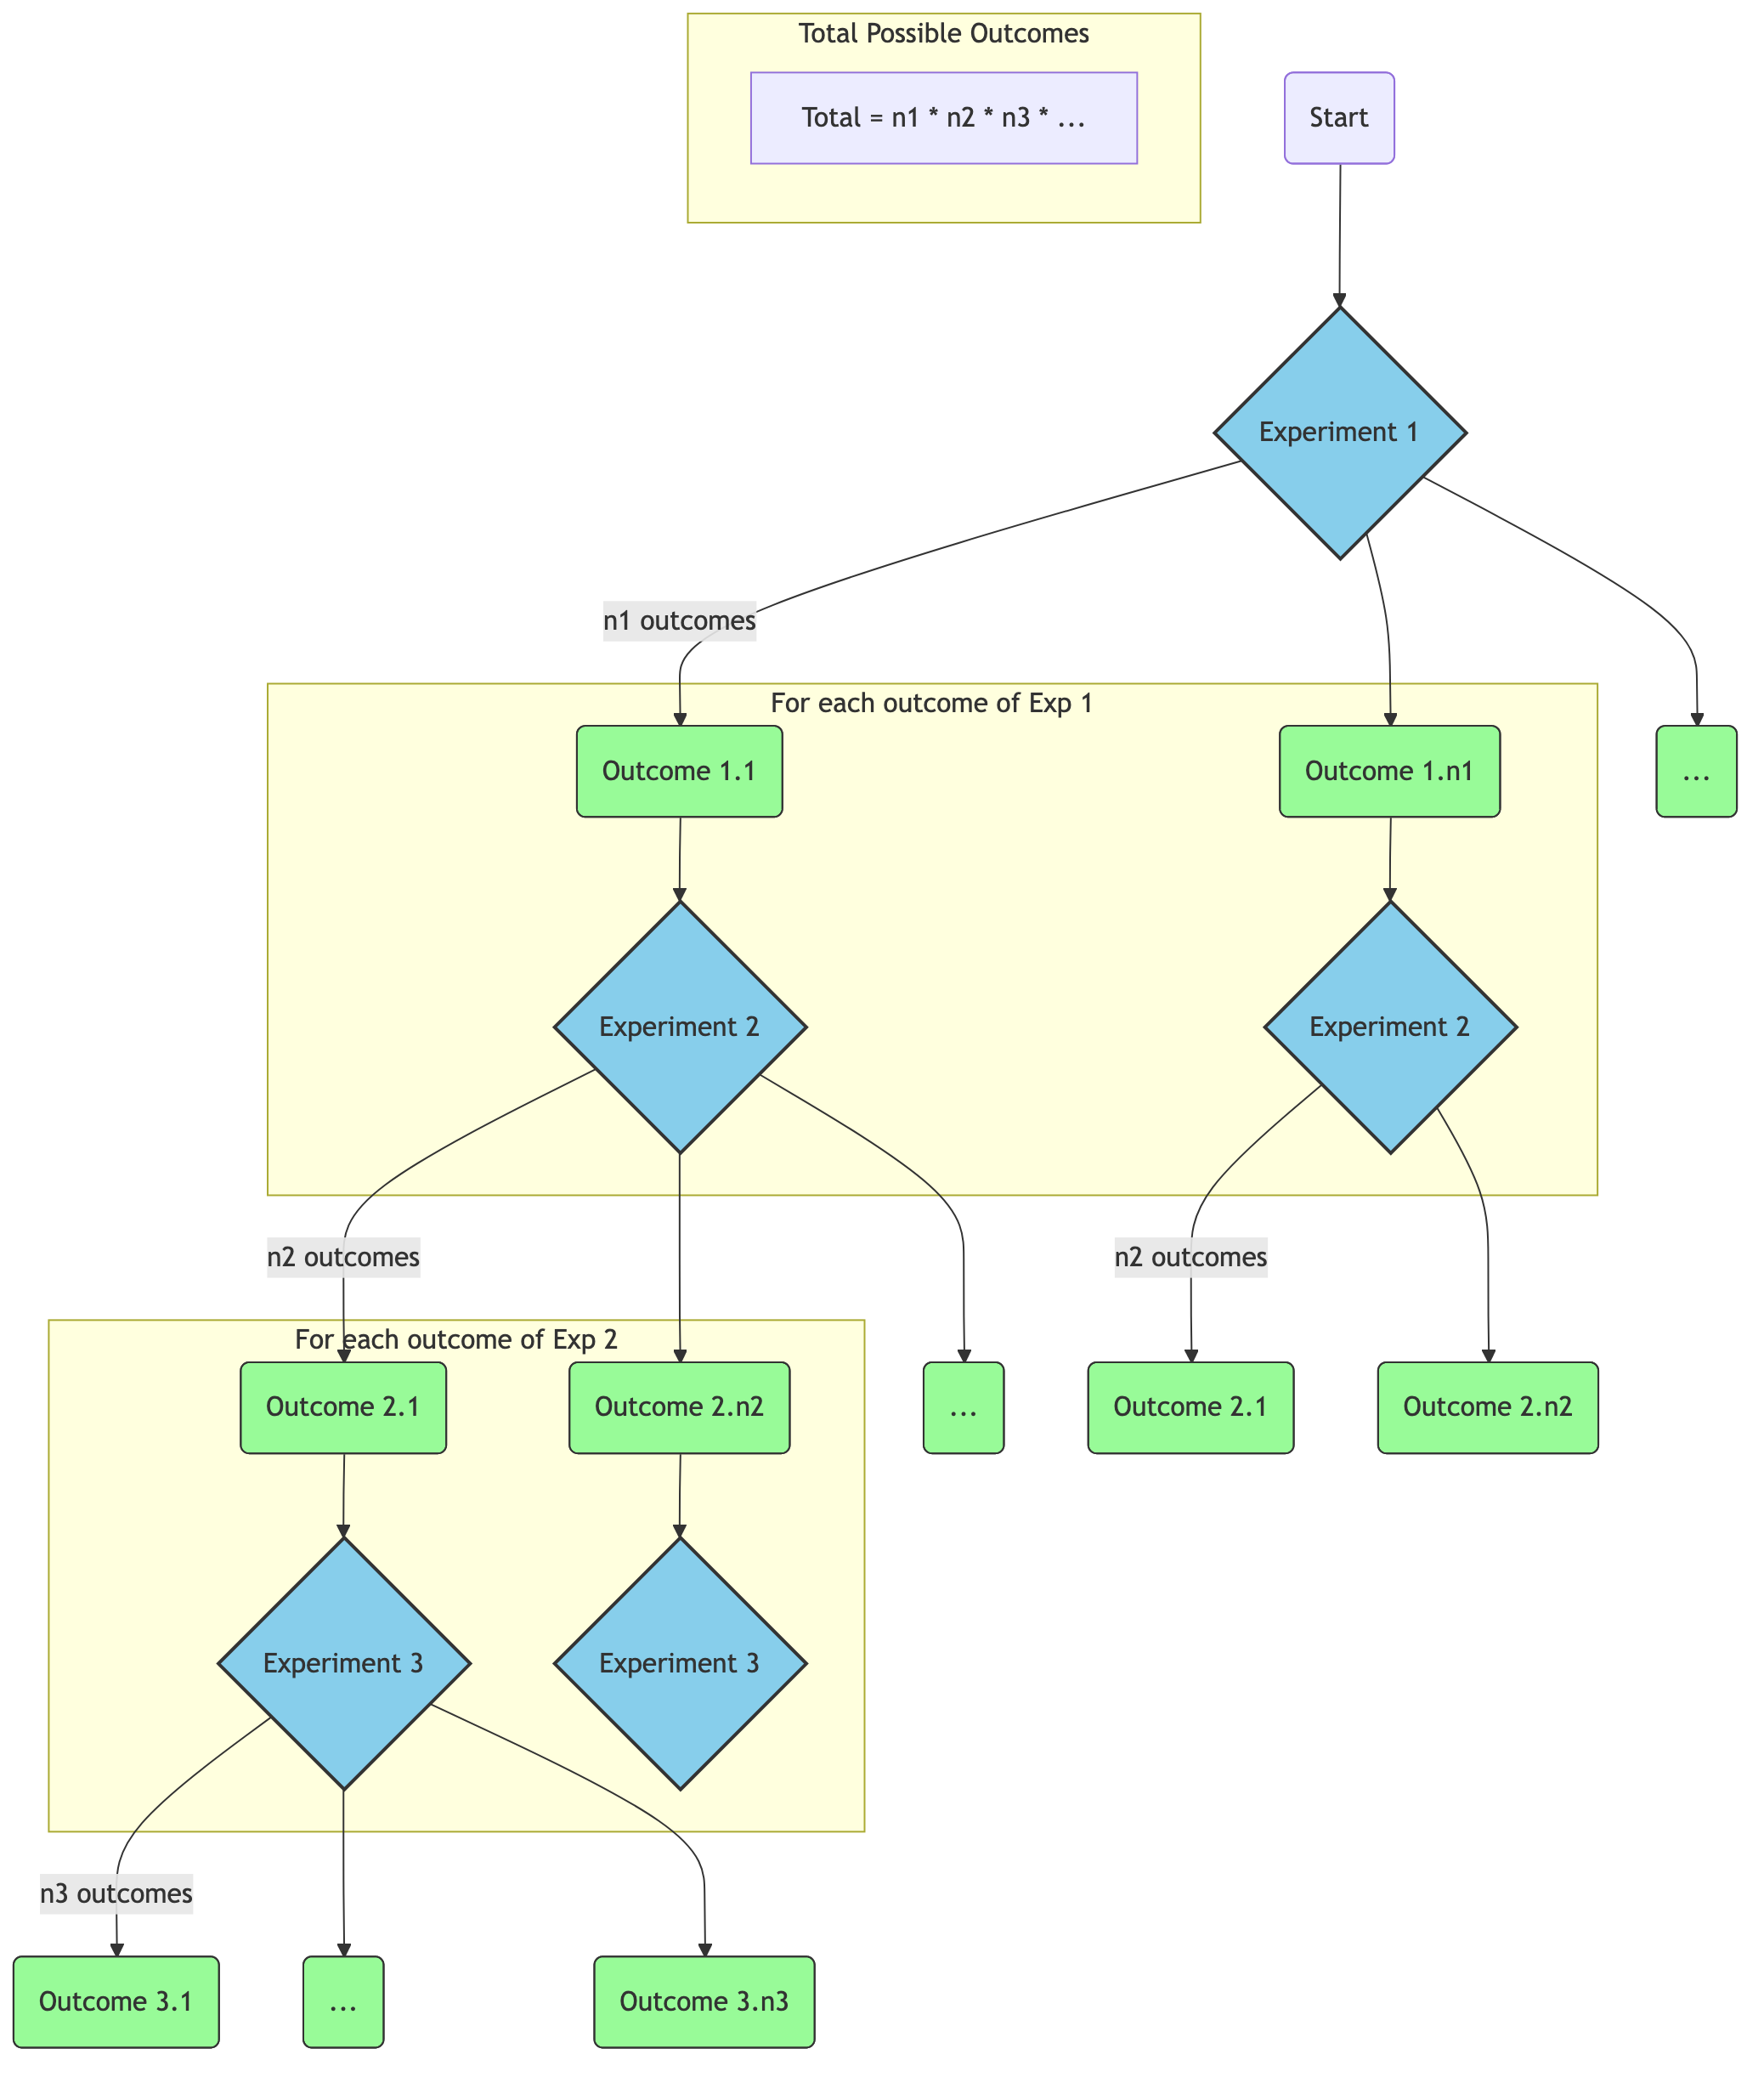
\includegraphics[width=0.8\textwidth]{counting.png}
    \caption{Mermaid diagram illustrating the Generalized Basic Principle of Counting}
    \label{fig:counting}
\end{figure}



\begin{examplebox}[title=Example: License Plates with Repetition]
    How many different \(7\) place license plates are possible if the first two places are to be occupied by letters and the remaining five by digits?
    
    \textbf{Solution:} The first two places can be filled with any of the \(26\) letters of the alphabet. Assuming letter can be repeated, the first place has \(26\) options and the second place has \(26\) options. The remaining five places can be filled with any of the \(10\) digits (from \(0\) to \(9\)), repeatedly. Therefore, the total number of different license plates is:

    \[
    26 \times 26 \times 10^5
    \]
\end{examplebox}

\begin{examplebox}[title=Example: License Plates without Repetition]
    If the letters and numbers in the previous example cannot be repeated, how many different license plates are possible?
    
    \textbf{Solution:} The first place has \(26\) options and the second place has \(25\) options (since letters cannot be repeated). The remaining five places can be filled with any of the \(10\) digits (from \(0\) to \(9\)). Therefore, the total number of different license plates is:

    \[
    26 \times 25 \times 10 \times 9 \times 8 \times 7 \times 6
    \]
\end{examplebox}

\section{Permutations}

\textbf{How many different ordered arrangements of letters \(a,b,c\) are possible?}

By enumeration we can see that : 

\[
abc, acb, bac, bca, cab, cba
\]
Each arrangement is called a \textbf{permutation} of the letters \(a,b,c\). There are \(6\) possible permutations for \(3\) distinct letters or a set of \(3\) distinct objects.

\begin{definitionbox}
    A permutation of \(n\) distinct objects is an arrangement of the objects in a specific order. The number of permutations of \(n\) distinct objects is given by \(n!\) (n factorial), which is the product of all positive integers up to \(n\):
    
    \[
    n! = n \times (n-1) \times (n-2) \times \ldots \times 2 \times 1
    \]
\end{definitionbox} 

\begin{keyconceptbox}
Let us start with \(n\) different objects and \(k\) be a positive integer such that \(k \leq n\). We want to determine the number of ways in which we can pick \(k\) objects from the total of \(n\) objects and arrange them in a sequence. i.e. the number of distinct \(k\) object sequence. We can do it in the following way 

\begin{itemize}
    \item We can pick the first object in \(n\) ways
    \item We can pick the second object in \(n-1\) ways (since we cannot pick the first object again)
    \item We can pick the third object in \(n-2\) ways (since we cannot pick the first and second objects again)
    \item ...
    \item We can pick the \(k\)-th object in \(n-(k-1)\) ways (since we cannot pick the first \(k-1\) objects again)
\end{itemize}

Therefore, by the generalized basic principle of counting, the total number of ways in which we can pick \(k\) objects from the total of \(n\) objects and arrange them in a sequence is given by
\begin{align*}
    n \times (n-1) \times (n-2) \times \ldots \times (n-(k-1)) &= \frac{n \times (n-1) \times (n-2) \times \ldots \times (n-(k-1)) \times (n-k) \times (n-(k+1)) \times \ldots \times 2 \times 1}{(n-k) \times (n-(k+1)) \times \ldots \times 2 \times 1} \\
    &= \frac{n!}{(n-k)!}
\end{align*}
In a special case when \(k=n\), we have
\[ \frac{n!}{(n-n)!} = \frac{n!}{0!} = n! \]
which is the number of ways in which we can arrange \(n\) distinct objects in a sequence.
\end{keyconceptbox}

